
\documentclass{article}

\usepackage{graphicx}

%-------------------------------------------------------------------------
\begin{document}

\title{2-D Wave Equation}
\author{ Isaac Dooley }



\maketitle

The wave equation can be stated in the following form, 
\begin{equation}
\frac{\partial^2p}{\partial p^2}=c^2 \nabla^2 p ,\label{PDE}
\end{equation}
where p is a physical measure such as a pressure, or the height of the water in a tub. This equation can be discretized over a 2d grid using a finite differencing scheme. Assume the pressures are located across a rectangular 2-D grid in x and y dimensions. We call the value of the pressure $p_{x,y}^{t}$ for time $t$ at location $\left(x,y\right)$ in the grid. One solution to the differential equation (\ref{PDE}) is the following:

\begin{equation}
p_{x,y}^{t+1} + p_{x,y}^{t-1} -2 p_{x,y}^{t} = c^2 \left(p_{x+1,y}^{t}+p_{x-1,y}^{t}+p_{x,y+1}^{t}+p_{x,y-1}^{t}-4p_{x,y}^{t}\right).\label{DISC}
\end{equation}

The left hand side term $\frac{\partial^2p}{\partial p^2}$ is represented in terms of the values of $p$ at three consecutive timesteps at grid location $\left(x,y\right)$. The right hand side terms are discretized using the $p$ values for the 4 locations adjacent to $\left(x,y\right)$ in the grid. One can simply solve for $p_{x,y}^{t+1}$ in equation (\ref{DISC}) to produce an update rule, 

\begin{equation}
p_{x,y}^{t+1} = c^2 \left(p_{x+1,y}^{t}+p_{x-1,y}^{t}+p_{x,y+1}^{t}+p_{x,y-1}^{t}-4p_{x,y}^{t}\right)- p_{x,y}^{t-1} +2 p_{x,y}^{t} .
\end{equation}

This update rule specifies how the $p$ value for each location in the grid should be computed, using $p$ values from the two previous time steps. This update rule is easy to code in an application. The application simply maintains two timesteps' worth of $p$ grids, and using these, the next timestep's $p$ grid can be computed. The $c$ term determines the wave speed. This value must be small enough such that the wave cannot move across more than one grid square in a single timestep. Smaller values for $c$ will make the simulation take longer to propagate a wave by a fixed distance, but larger values for $c$ can introduce dispersive and diffusive errors.


\begin{figure}
\begin{center}
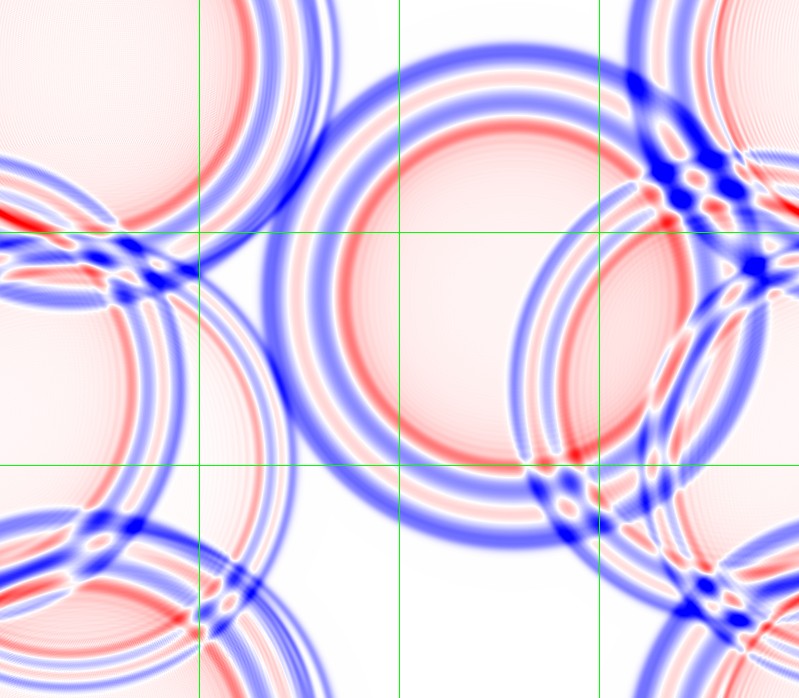
\includegraphics[width=5in]{screenshot}
\caption{A screenshot of the wave2d program. Positive values of $p$ on the grid are colored red, while negative values are colored blue. The green lines show the parallel decomposition of the problem onto a 4x4 chare array.
\label{screenshot}}
\end{center}
\end{figure} 


\end{document}

